% !TEX root = ../main.tex
\paragraph{Central Vertex Tracker (CVT)}
\label{par::cvt}
    The Central Vertex Tracker (CVT) system is an integral part of the CLAS12 CD.
    It is primarily used for measuring the momentum and determining the vertex position of charged particles scattered from the target.

    The CVT system is located inside the solenoid magnet, as depicted in figure \ref{fig::cvt}.
    It consists of two distinct detectors: the Silicon Vertex Tracker (SVT) and the Barrel MicroMegas Tracker (BMT).

    The SVT system is composed of three regions, each equipped with double-sided modules of silicon sensors.
    The regions have different numbers of modules: 10, 14, and 18, respectively.
    These silicon sensors are instrumented with a digital Application-Specific Integrated Circuit (ASIC) readout.
    The readout pitch, which refers to the distance between adjacent readout channels, is approximately 156 micrometers.
    Overall, the SVT system comprises 21,504 channels \cite{antonioli2020}.

    \begin{wrapfigure}{r}{0.50\textwidth}
        \centering\frame{
        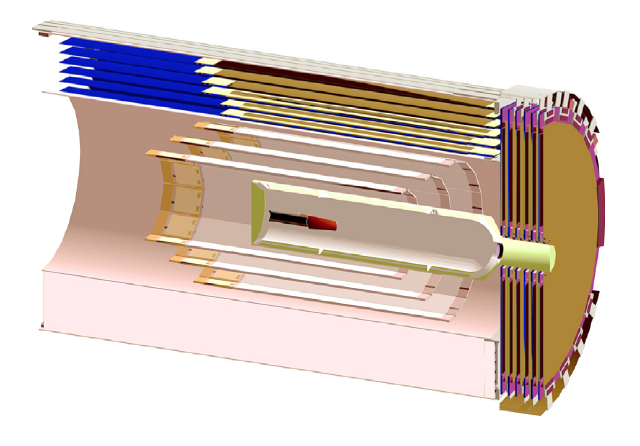
\includegraphics[width=\linewidth]{221cvt.png}}
        \caption[CVT]{Render of the Central Vertex Tracker.
        From the inside, the figure shows the target cell and vacuum chamber, the three double layers of the SVT, followed by the six layers of the BMT.
        The beam enters from the left.
        The six FMT layers are shown at the downstream end at the right.
        Source: \hyperlink{jlab.org/physics/hall-b/clas12}{CLAS12 wiki}.}
        \label{fig::cvt}
    \end{wrapfigure}

    The BMT is composed of three layers of strips aligned along the beamline and three layers of circular readout strips around the beamline, totalling 15,000 readout elements.
    It significantly enhances momentum resolution and tracking efficiency.
    Each layer is divided azimuthally into three segments, providing $120\degree$ azimuthal coverage for each segment.
    The system is designed to operate at the full luminosity of $10^{35} \text{cm}^{-2}\text{s}^{-1}$ \cite{acker2020mvt}.
